\documentclass[border=2pt]{standalone}
\usepackage{tikz}
\usepackage{pgfplots,pgfplotstable}
\pgfplotsset{compat=1.8}
\usetikzlibrary{positioning}

\graphicspath{{../paperFigures/}}
\input{../../defineBreastGTlabelColors.tex}

\begin{document}
\newcommand\mySize{13cm}
% argument #1: any options
\newenvironment{customlegend}[1][]{%
    \begingroup
    % inits/clears the lists (which might be populated from previous
    % axes):
    \csname pgfplots@init@cleared@structures\endcsname
    \pgfplotsset{#1}%
}{%
    % draws the legend:
    \csname pgfplots@createlegend\endcsname
    \endgroup
}%
% makes \addlegendimage available (typically only available within an
% axis environment):
\def\addlegendimage{\csname pgfplots@addlegendimage\endcsname}

\begin{tikzpicture}



\tikzstyle{myLegendStyle} = [ align=left,
                              draw=none,
                              column sep=2ex,
                              font=\tiny,
                            ]

%\newcommand\addMyLegendArea[1][]
%  { \addlegendimage{#1,area legend} }
  
\begin{customlegend}
  [ legend columns=   5,
    legend style  =   myLegendStyle,
    legend entries= { Background,                 
                      Chest wall,        
                      Pectoral muscle,                         
                      Adipose tissue,       
                      Lesion,            
                      Air (or lungs),                   
                      Rib,                            
                      Fibro-glandular tissue,      
                      Skin,                         
                      Boundary,                            
                    },
    anchor = north,
    at = {(0,4)},
  ]

%  \addMyLegendArea{red}
  \addlegendimage{bgColor!50!black,         fill=bgColor,         area legend}
  \addlegendimage{chestWallColor!50!black,  fill=chestWallColor,  area legend}
  \addlegendimage{pectoralColor!50!black,   fill=pectoralColor,   area legend}
  \addlegendimage{fatColor!50!black,        fill=fatColor,        area legend}
  \addlegendimage{lesionColor!50!black,     fill=lesionColor,     area legend}
  \addlegendimage{lungColor!50!black,       fill=lungColor,       area legend}
  \addlegendimage{ribColor!50!black,        fill=ribColor,        area legend}
  \addlegendimage{fibroGlandColor!50!black, fill=fibroGlandColor, area legend}
  \addlegendimage{skinColor!50!black,       fill=skinColor,       area legend}
  \addlegendimage{boundaryColor!50!black,   fill=boundaryColor,   area legend}

\end{customlegend}

\node[anchor=south west,inner sep=0] (imgNode) at (-11.5,1.5) {\includegraphics[width=\mySize]{pngImgs/gt/000002.png}};

\node[anchor=south east,inner sep=0] at (-12,1.5) {\includegraphics[width=\mySize]{pngImgs/000002.png}};

\end{tikzpicture}
\end{document}
